\section{Theorie}
\label{sec:Theorie}

\subsection{Zielsetzung und Gruundlagen}
    In diesem Versuch wird mittels eines Ultraschallgeräts die Fließgeschwindigkeit von einem 
    speziellen Flüssigkeitsgemisch innerhalb von Schläuchen verschiedener Durchmesser
    bestimmt. Dazu wird der Dopplereffekt verwendet. Treffen Schallwellen auf einen bewegten Körper,
    ist die Frequenz der reflektierten Schallwellen verändert. Bewegt sich der Körper auf die 
    Schallwelle zu, verschiebt sich die Frequenz in den höheren Bereich; entfernt sich der Körper
    von der Quelle der Schallwellen, sinkt die Frequenz. Die Frequenz der reflektierten Welle 
    beträgt
    \begin{equation}
        f_{kl/gr}=\dfrac{f_0}{1\pm \dfrac{v}{c}}.
    \end{equation}
    Diese Eigenschaft wird verwendet, um die Fließgeschwindigkeit zu bestimmen. Dazu wird eine 
    Sonde verwendet, die sowohl Ultraschallwellen aussendet, als auch die reflektierten Wellen 
    misst. Diese wird wie in Abbildung dargestellt, unter einem bestimmen Winkel auf das zu 
    untersuchende Medium gerichtet. Wie zuvor beschrieben, wird die reflektierte Schallwelle
    frequenzverschoben. Der Zusammenhang zu dem Winkel $\alpha$ der Sonde zu dem Schlauch 
    lautet
    \begin{equation}
        \Delta f = 2 f_0 \dfrac{v}{c} \cos{\alpha}
    \end{equation}
    wobei v die Geschwindigkeit der Flüssigkeit darstellt und c die Schallgeschwindigkeit in 
    dem Medium wie in Abbildung \ref{fig:KeineAhnung2} dargestellt.
    \begin{figure}
        \centering
        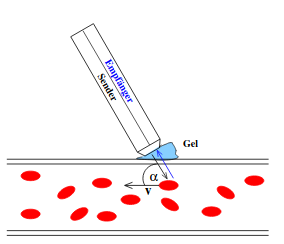
\includegraphics{US3.png}
        \caption{Darstellung der Ultraschallsonde}
        \label{fig:KeineAhnung2}
    \end{figure}

\subsection{Ultraschall}
    Als Ultraschall wird der Schall bezeichnet, dessen Frequenz über der vom Menschen wahrnehmbaren 
    Schwelle, d.h. über 20 kHz liegt. Um Ultraschall zu erzeugen wird sich der piezo-elektrische
    Effekt zu Nutzen gemacht. Dabei wird ein Piezokristall in ein elektrisches Wechselfeld eingebettet
    und dadurch zum Schwingen angeregt. Wird die Eigenfrequenz des Kristalls getroffen, kommen
    große Schwingungsamplituden zustande, so dass Ultraschallwellen mit hoher Schallenergiedichte 
    erzeugt werden. Das selbe Prinzip kommt beim Empfangen der reflektierten Schallwelle zum 
    tragen.
